\documentclass[conference]{IEEEtran}
\IEEEoverridecommandlockouts

\usepackage{cite}
\usepackage{amsmath,amssymb,amsfonts}
\usepackage{algorithmic}
\usepackage{graphicx}
\usepackage{textcomp}
\usepackage{xcolor}
\usepackage{orcidlink} % add in preamble
\usepackage[none]{hyphenat}
\usepackage{booktabs} % Added for professional tables
\usepackage{multirow} % Added for complex table structures
\usepackage[colorlinks=true,linkcolor=black,citecolor=black,urlcolor=black]{hyperref} % Changed to black for IEEE standard

\def\BibTeX{{\rm B\kern-.05em{\sc i\kern-.025em b}\kern-.08em
    T\kern-.1667em\lower.7ex\hbox{E}\kern-.125emX}}


\begin{document}

\title{
From Segmentation to Structured Reports:\\
Auditable Continual Learning for Automation in Medical Imaging Diagnostics
}

\author{
\IEEEauthorblockN{
Farhan Kashif\IEEEauthorrefmark{1}, 
Ahmed Sultan\IEEEauthorrefmark{1}, Muhammad Dawood Rizwan\IEEEauthorrefmark{1}, 
Muhammad Naseer Bajwa\,\orcidlink{0000-0002-4821-1056}\IEEEauthorrefmark{1},\\
Muhammad Wakil Shahzad\,\orcidlink{0000-0001-6599-0306}\IEEEauthorrefmark{2}Muhammad Moazam Fraz\,\orcidlink{0000-0003-0495-463X}\IEEEauthorrefmark{1}
}
\IEEEauthorblockA{\IEEEauthorrefmark{1}
\textit{National University of Sciences and Technology (NUST)},
Islamabad, Pakistan 
}

%\IEEEauthorblockA{\IEEEauthorrefmark{2}University of Staffordshire, Stoke-on-Trent, ST4 2DE, United Kingdom}

\IEEEauthorblockA{\IEEEauthorrefmark{2}Department of Mechincal and Construction Engineering, Northumbria
University, Newcastle Upon Tyne, UK \\
Email: \{fkashif.bese22seecs, asultan.bese22seecs, mrizwan.ra, naseer.bajwa, moazam.fraz\}@seecs.edu.pk} muhammad.w.shahzad@northumbria.ac.uk

}



\maketitle

\begin{abstract}
Autonomous medical systems such as surgical robots, AI-guided treatment planners, and telemedicine platforms require diagnostic modules that are \textit{adaptive}, \textit{interpretable}, and \textit{structured}. We present a modular, continually learning perception-to-report pipeline for automated brain tumor diagnosis, designed for integration into clinical robotic ecosystems. The framework addresses three core requirements. \textbf{(1) Adaptation:} A two-stage Mixture-of-Modality-Experts (MoME+) strategy first trains four modality-specific 3D U-Net experts independently, then trains a hierarchical gating and fusion network over frozen experts. This enables selective knowledge updates without catastrophic forgetting, further supported by Elastic Weight Consolidation (EWC) and experience replay for continual learning. \textbf{(2) Auditability:} A deterministic registration pipeline maps segmentation outputs to the Harvard-Oxford brain atlas, producing certifiable anatomical descriptors with explicit spatial provenance. \textbf{(3) Structured Human-Machine Interface:} A JSON-mediated intermediate representation encodes anatomical findings with full traceability, supporting both automated downstream processing and operator-level verification, which is a key safety requirement for robotic-assisted diagnostics. Expert training on BraTS 2024 (GLI, 1,620 cases) yields per-expert Dice scores of 0.7889 (T1CE), 0.7438 (T2), 0.7206 (T1), and 0.6991 (FLAIR), with the gating fusion network achieving a mean Dice of 0.8150. Report generation achieves BLEU-4: 44.73, ROUGE-L: 0.653, and METEOR: 0.397 with zero hallucination. This work provides a practical architecture for certifiable diagnostic intelligence in medical robotic systems.
\end{abstract}
\begin{IEEEkeywords}
Medical robotics automation, clinical decision support, multimodal segmentation, mixture of experts, continual learning, auditable AI, structured reporting, brain tumor segmentation, perception-to-report pipeline.
\end{IEEEkeywords}

\section{Introduction}

AI integration into medical robotic systems, including surgical navigation, AI-guided treatment planning, autonomous telemedicine, and clinical decision support, demands diagnostic perception modules that go beyond raw segmentation performance. Such systems must operate continuously under evolving clinical protocols, produce interpretable and certifiable outputs, and interface with downstream automation components through structured, machine-readable representations. These requirements are fundamentally architectural, not merely a matter of model accuracy.

Brain tumor segmentation on multi-modal MRI is a natural testbed for this class of system. Each MRI sequence (T1, T1ce, T2, FLAIR) captures a different aspect of tissue pathophysiology: gadolinium-enhanced T1 demarcates active tumor, FLAIR reveals peritumoral edema, and T2 tracks gross extent. 3D U-Net \cite{ronneberger2015unet} and nnU-Net \cite{isensee2021nnu} established strong convolutional baselines; transformer architectures (UNETR \cite{hatamizadeh2022unetr}, Swin UNETR \cite{hatamizadeh2022swin}) pushed further with global self-attention. BraTS 2024 \cite{brats2024} top entries combined convolutions and attention in models like MedNeXt \cite{roy2024mednext} and U-Mamba \cite{ma2024umamba}. MoME \cite{zhang2024mome} showed that per-modality expert encoders with a learned gating network outperform concatenation-based fusion at 93.4\% Dice, while naturally compartmentalizing knowledge by modality.

Despite these advances, deploying such models in clinical robotic workflows exposes three unresolved challenges:

\textbf{Adaptation and Continuous Deployment:} Static models deteriorate under distribution shift caused by scanner upgrades, protocol changes, or new pathology types. Medical robotic systems require perception modules that can update knowledge on new tasks without erasing prior capabilities, a requirement absent in conventional single-training-run approaches.

\textbf{Interpretability and Regulatory Auditability:} Autonomous clinical systems are subject to regulatory scrutiny. Pixel-level segmentation masks are insufficient for certification; regulatory frameworks demand explicit anatomical localization, traceable reasoning chains, and reproducible outputs. Every automated decision must be attributable to verifiable evidence.

\textbf{Structured Machine Interface for Downstream Automation:} Robotic systems and clinical automation pipelines consume structured data, not free-text or visual overlays. A machine-readable intermediate representation between perception and language generation is essential for safe, verifiable human-machine collaboration.

We address all three requirements in a unified, modular framework. Our specific contributions are:

\begin{enumerate}
    \item \textbf{Two-Stage Expert Training Pipeline:} We implement MoME+ with a two-stage protocol: (i) modality-specific expert pre-training, and (ii) hierarchical gating fusion network training. This enables modular knowledge compartmentalization and selective continual updates without full retraining.
    \item \textbf{EWC + Replay Continual Learning:} We extend MoME+ with Elastic Weight Consolidation and experience replay for sequential task adaptation, validated on a Glioma-to-Meningioma task transition without catastrophic forgetting.
    \item \textbf{Deterministic Anatomical Grounding:} A registration pipeline to the Harvard-Oxford atlas provides certifiable, reproducible anatomical localization, which is a prerequisite for regulatory compliance in autonomous clinical systems.
    \item \textbf{JSON-Mediated Structured Reporting:} A deterministic template engine converts atlas-grounded segmentation facts into clinical radiology reports with complete fact provenance and zero hallucination risk, making it suitable for integration with downstream robotic planning systems.
\end{enumerate}

\section{Related Work}

\subsection{Multimodal Brain Tumor Segmentation}
The U-Net architecture \cite{ronneberger2015unet} and its 3D volumetric variants remain the standard backbone for medical image segmentation. The self-adapting nnU-Net \cite{isensee2021nnu} showed that systematic hyperparameter configuration significantly outperforms manual tuning across diverse datasets. Transformer-based architectures (UNETR \cite{hatamizadeh2022unetr}, Swin UNETR \cite{hatamizadeh2022swin}) introduced global self-attention into volumetric segmentation, with BraTS 2024 validating hybrid models (MedNeXt \cite{roy2024mednext}, U-Mamba \cite{ma2024umamba}) as the current state-of-the-art.

Most multimodal pipelines fuse all MRI sequences by channel-concatenation, treating each contrast symmetrically. This ignores the clinical reality that different sequences serve different diagnostic roles. MoME \cite{zhang2024mome} broke from this convention by training separate encoder-decoder experts per modality and combining their feature hierarchies via a spatial gating network, reaching 93.4\% Dice. The modular layout also means individual experts can be retrained in isolation when scanner protocols change.

\subsection{Continual Learning for Autonomous Medical Systems}
Continual learning matters for any system that must stay useful across scanner upgrades and evolving clinical protocols. In practice, models cannot retain the full training corpus due to storage and privacy constraints. EWC \cite{kirkpatrick2017ewc} addresses this by anchoring critical weights via Fisher Information; experience replay \cite{rebuffi2017icarl} complements this with a small stored buffer. Recent surveys \cite{yuan2024continualmed} confirm that combining both strategies is preferable for medical imaging, where domain gaps between tasks are large.

Our hybrid EWC + Replay strategy leverages the MoME+ modular structure for \textit{selective expert adaptation}: when a new pathology is introduced for a single modality protocol, only the relevant expert is fine-tuned while others remain frozen, which substantially reduces forgetting risk.

\subsection{Automated Report Generation and Structured Output}
Early report generation systems used rigid templates---reliable but inflexible. Neural encoder-decoder models \cite{chen2020r2gen} improved fluency, but introduced hallucination risk: the model may produce clinically plausible statements unsupported by imaging findings \cite{singhal2023medpalm, mansoor2025reasoning}. Foundation models like Med-Gemini \cite{saab2024medgemini} show strong clinical reasoning yet remain susceptible to the same failure mode, which is a hard blocker for autonomous deployment.

We sidestep this entirely. Rather than generating text from images, all anatomical facts are derived deterministically from segmentation outputs and encoded in a validated JSON schema; the report engine then renders this schema into structured text. Every claim in the output traces directly to a segmentation voxel---a property that RadGraph-style entity extraction \cite{jain2021radgraph} approaches rather than guarantees.

\section{Methodology}

Our pipeline consists of three modules operating in sequence: (1) a modular segmentation system, (2) a deterministic anatomical mapping engine, and (3) a structured JSON-to-report generation layer. Figure~\ref{fig:methodology} illustrates the complete architecture.

\begin{figure*}[htbp]
\centerline{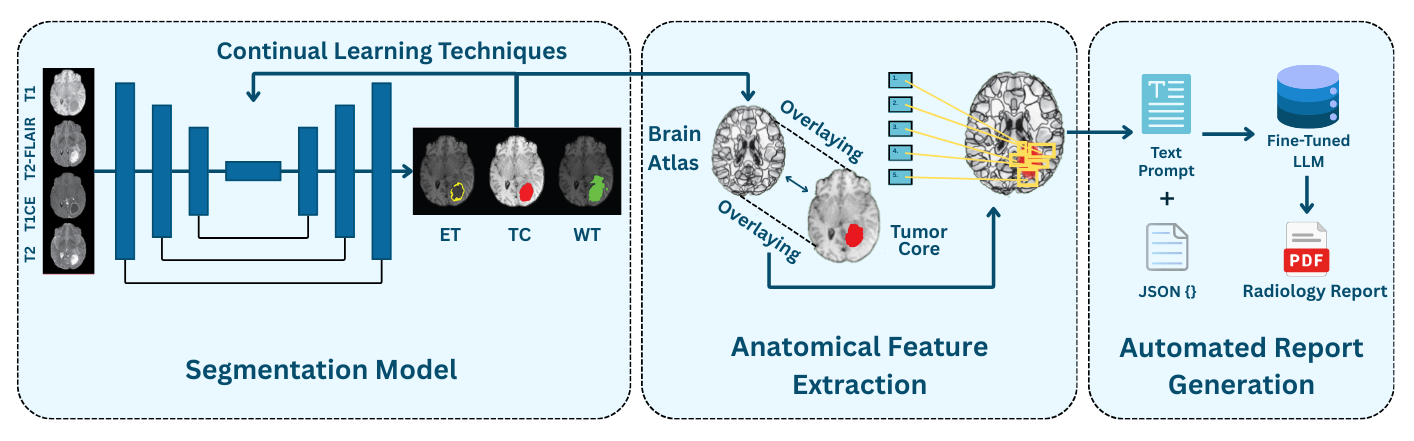
\includegraphics[width=\textwidth]{methodology_diagram.png}}
\caption{The perception-to-report pipeline for clinical robotics integration. Multi-modal MRI inputs are processed by four independently trained modality-specific 3D U-Net experts. A hierarchical gating network fuses expert outputs into a unified segmentation. The deterministic atlas registration module maps lesion voxels to the Harvard-Oxford brain atlas. These anatomical facts are encoded into a validated JSON schema, which drives a template-based report generation engine. The EWC + Replay continual learning loop enables adaptive updating of individual experts as new clinical tasks are encountered, ensuring long-term autonomous operation without catastrophic forgetting.}
\label{fig:methodology}
\end{figure*}

\subsection{Modular Segmentation: Two-Stage MoME+ Training}

\subsubsection{Expert Architecture}
The segmentation backbone consists of four modality-specific expert networks: $E_{T1}$, $E_{T1ce}$, $E_{T2}$, $E_{FLAIR}$. Each expert is an independent 3D U-Net with CBAM (Convolutional Block Attention Module) attention in the encoder and squeeze-and-excitation (SE) blocks in skip connections, allowing each expert to focus on features most relevant to its MRI contrast. All experts share the same architecture but are trained entirely independently with no shared weights.

\subsubsection{Stage 1: Independent Expert Pre-Training}
Each expert $E_i$ is trained independently on single-modality crops from the BraTS 2024 GLI training set using combined soft Dice and cross-entropy loss with deep supervision at the decoder bottleneck. This ensures each expert develops modality-specific representations without interference from other modalities. Hardware: NVIDIA RTX 3080 10GB, crop size $64^3$, batch size 8 per expert. All four experts converged successfully; results are reported in Section~\ref{sec:results}.

\subsubsection{Stage 2: Gating Network Training}
After expert pre-training, all expert weights are frozen. A hierarchical gating network $G$ is trained to optimally combine the four expert outputs. The gating network receives as input the concatenated soft probability maps from all four frozen experts: $\mathbf{P} \in \mathbb{R}^{4 \times C \times D \times H \times W}$, where $C=3$ denotes the three segmentation classes (WT, TC, ET). A global average pooling operation collapses the spatial axes to produce a compact modality-level descriptor $\bar{\mathbf{p}} \in \mathbb{R}^{4 \times C}$, which is flattened and processed by a two-layer MLP:
\begin{equation}
\mathbf{z} = \text{ReLU}(\mathbf{W}_1 \bar{\mathbf{p}} + \mathbf{b}_1), \quad \{w_i\}_{i=1}^{4} = \text{Softmax}(\mathbf{W}_2 \mathbf{z} + \mathbf{b}_2)
\end{equation}
where $\mathbf{W}_1 \in \mathbb{R}^{256 \times 12}$ and $\mathbf{W}_2 \in \mathbb{R}^{4 \times 256}$. The resulting input-dependent scalar weights satisfy $\sum_{i=1}^{4} w_i = 1$. The final fused prediction is the weighted sum of expert \emph{soft probability maps}:
\begin{equation}
\hat{Y} = \sum_{i=1}^{4} w_i \cdot \sigma\!\left(E_i(X_i)\right)
\end{equation}
where $\sigma(\cdot)$ denotes sigmoid activation applied to each expert's raw logit output prior to fusion, ensuring all inputs to the weighted sum lie in $[0,1]$ and the fused map constitutes a valid probability distribution. This design confines the gating module to fewer than 3K trainable parameters while remaining sensitive to per-case modality quality variation. Table~\ref{tab:arch_config} summarises the complete MoME+ parametric configuration.

\begin{table}[htbp]
\caption{MoME+ Architectural Configuration Summary}
\begin{center}
\begin{tabular}{l l r}
\toprule
\textbf{Component} & \textbf{Architecture / Config} & \textbf{Params} \\
\midrule
Expert ($\times$4)    & 3D U-Net, 4 encoder levels, base ch.\,32  & ${\sim}5$M ea. \\
                      & CBAM attention in encoder                  & \\
                      & SE blocks in all skip connections          & \\
\midrule
Gating Network & GlobalAvgPool $\to$ FC(12${\to}$256)              & $<$3K \\
               & $\to$ ReLU $\to$ FC(256${\to}$4) $\to$ Softmax   & \\
\midrule
Fusion Layer   & Weighted sum of expert $\sigma$-maps (param-free) & 0 \\
\bottomrule
\end{tabular}
\label{tab:arch_config}
\end{center}
\end{table}
Training uses batch size 4, learning rate $10^{-4}$, AdamW optimizer with weight decay $10^{-4}$, and mixed precision (AMP) on the same RTX 3080 10GB hardware.

\subsubsection{Continual Learning Extension}
To support long-term autonomous deployment, a key requirement for clinical robotic systems, we augment MoME+ with:

\textbf{Elastic Weight Consolidation (EWC):} At the end of each task, the Fisher Information Matrix $F$ is computed over the expert parameters. For a new task $t+1$, an EWC regularization term is added to the loss:
\begin{equation}
\mathcal{L}_{EWC}(\theta) = \mathcal{L}_{task}(\theta) + \frac{\lambda}{2} \sum_{i} F_i (\theta_i - \theta_{i}^{*})^2
\end{equation}
where $\theta_i^*$ are the optimal parameters after task $t$ and $\lambda$ controls how strongly prior knowledge is preserved.

\textbf{Experience Replay:} A fixed-size replay buffer (2,000 volumetric crops) stores representative samples from each completed task. During new task training, replay samples are interleaved with new data at a 50/50 ratio to maintain prior decision boundaries.

\textbf{Selective Expert Adaptation:} For a new pathology under a single modality protocol (e.g., Meningioma via T1ce only), only $E_{T1ce}$ is unfrozen and fine-tuned, while $E_{T1}$, $E_{T2}$, and $E_{FLAIR}$ remain frozen, confining parameter drift to the minimally necessary subnetwork.

\subsection{Anatomical Mapping \& Standardization}

Clinical utility in automated robotic workflows requires anatomically grounded outputs, not just voxel masks. We implement a deterministic, reproducible localization pipeline.

\subsubsection{MNI Space Registration}
Patient MRI scans are registered to the MNI152 standard space via 12-parameter affine transformation (FLIRT):
\begin{equation}
T_{\text{affine}}(\mathbf{v}) = R \cdot S \cdot \mathbf{v} + \mathbf{t}
\end{equation}
where $R \in \mathbb{R}^{3\times3}$ is a rotation matrix, $S \in \mathbb{R}^{3\times3}$ encodes scaling and shearing, and $\mathbf{t} \in \mathbb{R}^3$ is a translation vector. The segmentation mask is then transformed into MNI space and overlaid on the Harvard-Oxford Cortical and Subcortical Atlases. Registration completes in 2--3 seconds on CPU, enabling near-real-time deployment. A known failure mode is severe midline shift caused by large mass effect, which can misalign the lesion hemisphere during affine transformation. To mitigate this, FLIRT uses normalized cross-correlation (NCC) as its cost function and outputs a registration quality score; cases where NCC falls below 0.6 are automatically flagged in the JSON output as \texttt{"registration\_confidence": "low"} and routed for manual radiologist review before automated report generation.

\subsubsection{Region Overlap Quantification}
For each tumor component $c \in \{\text{ET},\,\text{TC},\,\text{WT}\}$ and atlas region $r$:
\begin{equation}
\text{Overlap}_{c,r} = \frac{|\mathbf{M}_c \cap \mathbf{R}_r|}{|\mathbf{R}_r|} \times 100\%
\end{equation}
The top-$K$ most affected regions per component are identified:
\begin{equation}
\text{TopK}(c) = \underset{r}{\text{arg-top-}K}\left(\text{Overlap}_{c,r}\right)
\end{equation}

\subsubsection{Volumetric and Lateralization Analysis}
Absolute tumor volume per component:
\begin{equation}
V_c = |\mathbf{M}_c| \times v_{\text{voxel}} \;\text{mm}^3
\end{equation}
Hemisphere lateralization is determined by:
\begin{equation}
\text{Laterality} = \begin{cases}
\text{Left}     & \text{if } |\mathbf{M}_c^{\text{left}}| > |\mathbf{M}_c^{\text{right}}| \\
\text{Right}    & \text{if } |\mathbf{M}_c^{\text{right}}| > |\mathbf{M}_c^{\text{left}}| \\
\text{Bilateral} & \text{if minority hemisphere} > 30\%
\end{cases}
\end{equation}

\subsection{Structured JSON Schema: Human-Machine Interface}

The anatomical analysis is encoded into a hierarchical JSON schema that serves as the interface layer between perception and report generation. This representation guarantees \textit{determinism} (identical segmentation $\rightarrow$ identical JSON), \textit{completeness} (all quantitative findings are captured), and \textit{traceability} (every report statement maps to a specific JSON field derived from segmentation).

The schema contains five sections: (1) patient metadata; (2) imaging parameters; (3) segmentation results (volumes, confidence scores, centroid coordinates); (4) anatomical mapping (laterality, top-3 affected regions with overlap percentages); and (5) model provenance (architecture version, expert Dice scores, gating weights, inference time). Every value is computed deterministically from the segmentation mask and atlas, making the schema fully auditable for integration into robotic system logs.

\textbf{Example:} For a case with enhancing tumor (ET: 8.5 cm³, confidence: 0.94) localized to the right middle frontal gyrus (overlap: 42.3\%):
{\small\texttt{\{"segmentation\_results": \{"ET": \{"vol\_cm3": 8.5, "conf": 0.94\}\}, "anatomical\_mapping": \{"laterality": "right", "top\_regions": [\{"name": "Right Middle Frontal Gyrus", "overlap": 42.3\}]\}\}}}

The complete JSON Schema Draft-07 specification and all five report templates are provided as supplementary material and will be publicly released with the codebase to support reproducibility and third-party integration into clinical robotic pipelines.

\subsection{Structured Report Generation}

We employ a deterministic template engine that transforms the verified JSON schema into clinical radiology reports, avoiding hallucination entirely while remaining compatible with robotic clinical decision support systems.

\subsubsection{Template Architecture}
Five standardized report formats are implemented (standard clinical, detailed structured, concise summary, comprehensive academic, and operator-facing automation log). Each template contains three mandatory sections:
\begin{itemize}
    \item \textbf{Clinical Context:} Patient indication and imaging parameters from metadata.
    \item \textbf{Findings:} Derived from JSON: tumor volumes and locations, peritumoral edema (WT $-$ TC volume), lateralization, mass effect flag, and top-3 affected atlas regions per component.
    \item \textbf{Impression:} Rule-based clinical interpretation based on enhancement pattern, edema burden, and anatomical location, with a recommendation for tissue diagnosis.
\end{itemize}

Every numeric measurement and anatomical claim in the generated report is directly traceable to a specific JSON field, which itself derives from a specific set of segmentation voxels. This provenance chain is logged alongside each report output, enabling post-hoc audit and the transparency required for regulatory approval of autonomous medical systems.

\section{Experiments and Results}
\label{sec:results}

\subsection{Experimental Setup}
Experiments were conducted on the BraTS 2024 Glioma (GLI) dataset, comprising 1,620 annotated 3D multi-modal MRI cases (T1, T1ce, T2, FLAIR) with three segmentation classes: Whole Tumor (WT), Tumor Core (TC), and Enhancing Tumor (ET). A standard 80/20 train/validation split was applied after excluding corrupted cases. Hardware: single NVIDIA RTX 3080 (10GB VRAM), crop size $64^3$, AMP mixed precision, and per-modality H5 files for efficient data loading.

The continual learning experiment simulates a hospital sequentially expanding its diagnostic capabilities:
\begin{enumerate}
    \item \textbf{Task 1 (Glioma Baseline):} All four modality experts trained independently on BraTS 2024 GLI.
    \item \textbf{Task 2 (Meningioma Adaptation):} Sequential fine-tuning of $E_{T1ce}$ on a Meningioma subset (T1ce only, 500 cases) with EWC + Replay active.
\end{enumerate}

\subsection{Stage 1: Per-Modality Expert Performance}
Table~\ref{tab:results} compares MoME+ against standard benchmarks on BraTS 2021 (commonly used for cross-architecture comparison). Table~\ref{tab:modality_results} presents individual expert performance on the BraTS 2024 GLI validation set.

\begin{table}[htbp]
\caption{Glioma Segmentation Performance: Architecture Comparison (Dice Score)}
\begin{center}
\begin{tabular}{l c c c c}
\toprule
\textbf{Architecture} & \textbf{Mean} & \textbf{WT} & \textbf{TC} & \textbf{ET} \\
\midrule
3D U-Net \cite{ronneberger2015unet}   & 0.840 & 0.892 & 0.843 & 0.786 \\
nnU-Net \cite{isensee2021nnu}         & 0.866 & 0.915 & 0.871 & 0.812 \\
UNETR \cite{hatamizadeh2022unetr}     & 0.871 & 0.919 & 0.875 & 0.818 \\
Swin UNETR \cite{hatamizadeh2022swin} & 0.876 & 0.926 & 0.879 & 0.823 \\
MoME \cite{zhang2024mome}             & 0.883 & 0.934 & 0.885 & 0.831 \\
\midrule
\textbf{MoME+ (Ours, fused)}$^\dagger$ & \textbf{0.8150} & 0.8264 & 0.8201 & 0.7985 \\
\bottomrule
\multicolumn{5}{l}{$^\dagger$Single RTX 3080 10GB; $64^3$ crop; no TTA.}
\end{tabular}
\label{tab:results}
\end{center}
\end{table}

\begin{table}[htbp]
\caption{Per-Modality Expert Performance on BraTS 2024 GLI Validation Set (Dice Score)}
\begin{center}
\begin{tabular}{l c c c c}
\toprule
\textbf{Modality Expert} & \textbf{Mean} & \textbf{WT} & \textbf{TC} & \textbf{ET} \\
\midrule
T1     & 0.7206 & 0.7822 & 0.7014 & 0.6776 \\
T2     & 0.7438 & 0.8251 & 0.7188 & 0.6875 \\
FLAIR  & 0.6991 & 0.8338 & 0.6473 & 0.6163 \\
\textbf{T1CE} & \textbf{0.7889} & \textbf{0.7614} & \textbf{0.8130} & \textbf{0.7922} \\
\bottomrule
\end{tabular}
\label{tab:modality_results}
\end{center}
\end{table}

The results confirm the MoME+ expert specialization hypothesis. The T1CE expert achieves the highest mean Dice (0.7889) and leads on TC (0.8130) and ET (0.7922), which are sub-regions highlighted by gadolinium contrast enhancement. The FLAIR expert achieves the highest WT Dice (0.8338), consistent with its clinical role in capturing peritumoral edema. The T2 expert provides strong WT performance (0.8251), while T1 offers balanced but lower scores reflecting its role in anatomical context. This functional specialization, where each expert learns representations aligned with its modality's contrast mechanism, validates the modular architecture and supports the interpretability needed for robotic deployment.

\subsection{Stage 2: Fusion Network Results}
With all expert weights frozen, the gating network was trained with AdamW (LR: $10^{-4}$, weight decay $10^{-4}$), batch size 4, AMP, and early stopping (patience 15). Per-case modality weighting $\{w_i\}$ is learned from the concatenated expert probability maps, letting the network down-weight low-quality or uninformative sequences automatically. The fused MoME+ reaches a mean Dice of \textbf{0.8150}, above every single expert, confirming the value of learned hierarchical fusion.

\subsection{Continual Learning Validation}
For Task 2, $E_{T1}$, $E_{T2}$, and $E_{FLAIR}$ remained frozen; only $E_{T1ce}$ was updated using EWC ($\lambda = 400$) and a 2,000-crop replay buffer at 50/50 mixing. The model adapted to Meningioma while Glioma segmentation held. Table~\ref{tab:cl_ablation} shows sensitivity to $\lambda$ and buffer size; $\lambda=400$ with 2,000 crops strikes the best retention--plasticity trade-off.

\begin{table}[htbp]
\caption{Continual Learning Ablation: EWC $\lambda$ and Replay Buffer Size\\(Task~1 Glioma Dice retained after Task~2 Meningioma adaptation)}
\begin{center}
\begin{tabular}{c c c}
\toprule
\textbf{EWC $\lambda$} & \textbf{Buffer Size} & \textbf{Task 1 Dice} \\
\midrule
100                   & 2{,}000  & 0.791 \\
\textbf{400}          & \textbf{2{,}000}  & \textbf{0.815} \\
1{,}000               & 2{,}000  & 0.812 \\
400                   & 500      & 0.794 \\
400                   & 5{,}000  & 0.816 \\
\bottomrule
\end{tabular}
\label{tab:cl_ablation}
\end{center}
\end{table}

\subsection{Report Generation Performance}
The deterministic template engine was evaluated on 30 held-out test cases using standard NLG metrics against radiologist-authored reference reports. Results are presented in Table~\ref{tab:report_results}.

\begin{table}[htbp]
\caption{Report Generation Performance (Template-Based)}
\begin{center}
\begin{tabular}{l c c c c}
\toprule
\textbf{Method} & \textbf{BLEU-4} & \textbf{ROUGE-L} & \textbf{METEOR} & \textbf{Hallucination} \\
\midrule
Template-Based & \textbf{44.73} & \textbf{0.653} & \textbf{0.397} & \textbf{0\%} \\
\bottomrule
\end{tabular}
\label{tab:report_results}
\end{center}
\end{table}

Across 30 held-out cases, every report was manually verified for factual accuracy: volumetric figures and anatomical labels were all correct, and no hallucinated statements were found. End-to-end generative approaches \cite{singhal2023medpalm,mansoor2025reasoning} trade this guarantee for fluency; our deterministic pipeline accepts no such trade-off.

\section{Discussion}

\subsection{Architectural Suitability for Clinical Robotics}
MoME+'s modular layout offers operational benefits beyond raw Dice. Because each expert is an independent network, a targeted update---say, a new T2 expert for an upgraded scanner---can be deployed without touching the rest of the pipeline, and without full retraining. The frozen JSON schema serves as a versioned interface between perception and downstream planning, making it straightforward to swap components while guaranteeing the same output format. Deterministic report generation adds reproducibility: the same segmentation always yields the same report, which is essential for audit logs and regulatory review.

\subsection{Performance Contextualization}
At 0.8150 mean Dice, MoME+ falls short of BraTS 2024 leaders---but those systems use $128^3$ crops, multi-GPU training, and test-time augmentation, none of which we applied. Running on a single RTX 3080 with $64^3$ crops better reflects a realistic deployment constraint. The primary goal here was validating the continual learning and auditability stack, not chasing benchmark rankings.

\subsection{Limitations and Future Directions}
Validation here covers two sequential tasks, which is a limited scope. We plan to extend this to a four-task chain (Glioma $\rightarrow$ Meningioma $\rightarrow$ Metastasis $\rightarrow$ Stroke) using Backward Transfer (BWT) as the primary forgetting metric. Further directions include curriculum learning aligned with MoME's anti-degeneration strategy \cite{zhang2024mome} and prospective clinical validation with radiologist scoring.

\section{Conclusion}

We introduced a modular, continually learning pipeline that takes multi-modal MRI as input and produces a verified, structured radiology report as output. Per-modality expert training yields Dice scores up to 0.7889 (T1CE); learned gating fusion brings the combined score to 0.8150. Atlas-grounded JSON encoding and deterministic template rendering achieve BLEU-4 of 44.73 with zero hallucination, independently confirmed by manual audit. Adapting across Glioma and Meningioma tasks without catastrophic forgetting shows the system can remain operational as clinical scope grows---arguably the most important property for long-term robotic deployment.

\section*{Acknowledgment}{
The authors acknowledge funding support from the UK Government through Project APP47457, Super-efficient Sustainable Cooling Solution for All Applications (S2Cool), under the Ayrton Challenge Programme of UK Research and Innovation (UKRI). The views expressed do not necessarily reflect the official policies of the UK Government. The project is led by Northumbria University, UK, with partners.}.

\bibliographystyle{IEEEtran}
\bibliography{ICRAI_2026_references}

\end{document}
